\appendix
\pagestyle{annexe}
% On change la numération des annexes en alphabétique
\renewcommand\thesection{\Alph{section}}
\setcounter{minitocdepth}{1} % Mini-toc breve (sections)
\chapter{Annexes}
\numberwithin{equation}{section}
\numberwithin{thm}{section}
\numberwithin{figure}{section}
\minitoc
\newpage
%% \begin{landscape}
\section{Tableaux des CIOE}

Nous rappelons l'expression des opérateurs \(\LD,\LR,\LL\) sur des champs vectoriels tangents
\begin{align*}
  \LD &= \vgrads{}\vdivs{} &
  \LR &= \vrots{} \vrots{} &
  \LL &= \vlapls{}
\end{align*}

Dans les codes numériques, tous les opérateurs sont normalisés par le carré du nombre d'onde dans le vide.

\begin{center}
\begin{tabular}{l|Cl}
Nom & \text{Expression sur les champs tangentiels} & Référence
\\
\hline
\hline
\hypertarget{ci0}{CI0} & \vE_t = a_0 \vJ  & \cite{leontovich_investigations_1948}
\\
\hypertarget{ci01}{CI01} & \vE_t = \left(a_0\oI + a_1 \LL \right)\vJ & \cite{stupfel_implementation_2015}
\\
\hypertarget{ci1}{CI1}& \left(\oI + b \LL \right)\vE_t = \left(a_0\oI + a_1 \LL \right)\vJ & \cite{stupfel_implementation_2015}
\\
\hypertarget{ci4}{CI4}& \vE_t = \left(a_0\oI + a_1 \LD - a_2 \LR \right)\vJ & \cite{hoppe_impedance_1995}
\\
\hypertarget{ci3}{CI3}& \left(\oI + b_1 \LD - b_2 \LR \right)\vE_t = \left(a_0\oI + a_1 \LD - a_2 \LR \right)\vJ & \cite{hoppe_impedance_1995}
\\
\hypertarget{ci6}{CI6}& \left(\oI + c_1 \LD - c_2 \LR \right)\vE_t = \left(\diag{a_1}{a_2} + b_1 \LD - b_2 \LR \right)\vJ & \cite{hoppe_impedance_1995}
\end{tabular}
\end{center}
% \end{landscape}
\newpage
\section{Formulation des équations de Maxwell}
\label{sec:annex:maxwell_equation}

Uniquement dans cette annexe, les constantes de matériaux relatives sont dénotées par l'indice \(~_r\).

Les équations de Maxwell temporelles sont
\begin{equation}
  \left\lbrace \begin{matrix}
  \vrot \vE + \mu \ddr{t}{\vect{H}} &=& 0,
  \\
  \vrot \vect{H} - \eps \ddr{t}{\vE} &=& 0.
  \end{matrix} \right.
\end{equation}

Donc les équations de Maxwell harmoniques en convention \(e^{i\w t}\) sont
\begin{equation}
  \left\lbrace \begin{matrix}
  \vrot \vE + i\w\mu \vect{H} &=& 0,
  \\
  \vrot \vect{H} - i\w\eps \vE &=& 0.
  \end{matrix} \right.
\end{equation}

On définit les constantes relatives \(\mu_r = \mu \slash \mu_0\), \(\eps_r = \eps \slash \eps_0\), \(k_0 = \w \sqrt {\eps_0\mu_0}\), \(\eta_0=\sqrt {\mu_0/\eps_0}\).

On pose \(\vH = \eta_0 \vect{H}\).
Les équations harmoniques se réécrivent
\begin{equation}
\left\lbrace \begin{matrix}
\vrot \vE + ik_0\eta_0\mu_r \vect{H} &= 0,
\\
\vrot \vect{H} - ik_0\eta_0^{-1}\eps_r \vE &= 0,
\end{matrix} \right.
\quad
\overset{\vH = \eta_0 \vect{H}}{\Rightarrow}
\quad
\left\lbrace \begin{matrix}
\vrot \vE + ik_0\mu_r \vH &= 0,
\\
\vrot \vH - ik_0\eps_r \vE &= 0.
\end{matrix} \right.
\end{equation}

On pose \(k=k_0\nu_r\), \(\nu_r = \sqrt{\mu_r\eps_r}\), \(\eta_r = \sqrt{\mu_r \slash \eps_r}\)

\begin{equation}
\left\lbrace \begin{matrix}
\vrot \vE + ik\eta_0\eta_r \vect{H} &= 0,
\\
\vrot \vect{H} - ik\eta_0^{-1}\eta_r^{-1} \vE &= 0,
\end{matrix} \right.
\quad
\overset{\vH = \eta_0 \vect{H}}{\Rightarrow}
\quad
\left\lbrace \begin{matrix}
\vrot \vE + ik\eta_r \vH &= 0,
\\
\vrot \vH - ik\eta_r^{-1} \vE &= 0.
\end{matrix} \right.
\end{equation}
\newpage
\section{Opérateurs gradient, divergent et rotationnel en coordonnées cartésiennes, cylindriques, sphériques et opérateurs surfaciques}
\label{sec:annexe:div_grad_rot}
\subsection{Cartésien}

    \begin{align}
        \vgrad f &= \ddr{x}{f}\vect{e_x} + \ddr{y}{f}\vect{e_y}  + \ddr{z}{f}\vect{e_z} \\
        \vdiv \vu &= \ddr{x}{u_x} + \ddr{y}{u_y} + \ddr{z}{u_z} \\
        \vrot\vu &= \left(\ddr{y}{u_z}-\ddr{z}{u_y}\right)\vect{e_x} + \left(\ddr{z}{u_x}-\ddr{x}{u_y}\right)\vect{e_y} + \left(\ddr{x}{u_y}-\ddr{y}{u_x}\right)\vect{e_z}
    \end{align}

\subsection{Cylindrique}

    \[
        (x,y,z) = (r\cos\theta,r\sin\theta,z)
    \]

    \begin{align}
        \vgrad f &= \ddr{r}{f}\vect{e_r}
        +\frac{1}{r}\ddr{\theta}{f}\vect{e_\theta} + \ddr{z}{f}\vect{e_z}
        \\
        \vdiv \vu &= \frac{1}{r}\ddr{r}{(ru_r)}+\frac{1}{r}\ddr{\theta}{u_\theta}+\ddr{z}{u_z}
        \\
        \vrot \vu &= \left(\frac{1}{r}\ddr{\theta}{u_z} - \ddr{z}{u_\theta}\right)\vect{e_r} +
        \left(\ddr{z}{u_r} - \ddr{r}{u_z}\right)\vect{e_\theta} +
        \frac{1}{r}\left(\ddr{r}{(ru_\theta)}-\ddr{\theta}{u_r}\right)\vect{e_z}
    \end{align}

\subsection{Sphérique}

    \[
        (x,y,z) = (r\cos\phi\sin\theta,r\sin\theta\sin\theta,r\cos\theta)
    \]

    \begin{align}
        \vgrad f &= \ddr{r}{f}\vect{e_r}
        +\frac{1}{r}\ddr{\theta}{f}\vect{e_\theta} + \frac{1}{r\sin\theta}\ddr{\phi}{f}\vect{e_\phi}
        \\
        \vdiv \vu &= \frac{1}{r^2}\ddr{r}{(r^2u_r)}
        + \frac{1}{r\sin\theta}\ddr{\theta}{}\left(\sin(\theta)u_\theta\right) + \frac{1}{r\sin\theta}\ddr{\phi}{u_\phi}
    \end{align}

    \begin{multline}
        \vrot \vu = \frac{1}{r\sin\theta}\left(\ddr{\theta}{}\left(\sin(\theta)u_\phi\right) - \ddr{\phi}{u_\theta}\right)\vect{e_r}\dots
        \\
        + \left(\frac{1}{r\sin\theta}\ddr{\phi}{u_r} - \frac{1}{r}\ddr{r}{(ru_\phi)} \right)\vect{e_\theta} \dots
        \\
        + \frac{1}{r}\left(\ddr{r}{(ru_\theta)}-\ddr{\theta}{u_r}\right)\vect{e_\phi}
    \end{multline}

\subsection{Opérateurs surfaciques}

    Soit \(\Omega\) un objet de surface \(\Gamma\) régulière et \(\vn\) la normale unitaire sortante de cet objet.
    Soit \(f\) et \(\vu\) une fonction et un champ de vecteurs dérivables en tout point \(\vx\) de \(\Gamma\), on rappelle de \cite{nedelec_acoustic_2001} les opérateurs différentiels surfaciques
    \begin{align}
        \vgrads{f}(\vx) &= \vgrad{f}(\vx) - \vn(\vx) (\vn(\vx) \cdot \vgrad{f}(\vx))
        \\
        \vdivs{\vu} &= \vdiv\left(\vu(\vx) - \vn(\vx) (\vn(\vx) \cdot \vu(\vx)\right)
        \\
        \vrots{\vu}(\vx) &= \vn(\vx)\left(\vn(\vx) \cdot \vrot{\vu}(\vx)\right)
    \end{align}
    Si l'on veut appliquer le rotationnel surfacique comme une application sur les champs tangentielles, les opérateurs rotationnel surfacique scalaire et rotationnel surfacique vectoriel
    \begin{align}
        \trots{\vu}(\vx) &= \vn(\vx) \cdot \vrot{\vu}(\vx)
        \\
        \tvrots{f}(\vx) &= - \vn \pvect \vgrads f(\vx)
    \end{align}
\newpage
\section[Solution dans le plan quand k3 = 0]{Solution dans le plan quand \(k_3 = 0\)}
  \label{sec:annexe:plan:k3_nul}

  Dans chaque couche de l'empilement plan.

  Si \(k_3 = 0\), \(k_x^2 + k_y^2 = w^2\eps\mu\) et il existe donc des constantes \((c_1(k_x,k_y),c_2(k_x,k_y))) \in \CC(\RR^2)^2\) telles que
  \begin{equation*}
    \hat{E_y}(k_x,k_y,z) = c_1(k_x,k_y) z + c_2(k_x,k_y)
  \end{equation*}

  Toute la méthode est aussi valable pour \(\hat H_y\), il existe des constantes \((c_3(k_x,k_y),c_4(k_x,k_y))) \in \CC(\RR^2)^2\) telles que
  \begin{equation*}
    \hat{H_y}(k_x,k_y,z) = c_3(k_x,k_y) z + c_4(k_x,k_y)
  \end{equation*}

  À partir des composantes \(\vect{e_x},\vect{e_y}\) des équations de Maxwell, on peut déterminer \(\hat{E_x},\hat{E_z},\hat{H_x},\hat{H_z}\).
  Cela revient à résoudre \(Y = \mM X\) où la matrice \(\mM\) et les vecteurs \(X, Y\) sont définis tels que
  \begin{align*}
    \mM =
    \begin{bmatrix}
    0 & -ik_y & -i\w\mu & 0
    \\
    ik_y & 0 & 0 & -i\w\mu
    \\
    i\w\eps & 0 & 0 & -ik_y
    \\
    0 & i\w\eps & ik_y & 0
    \end{bmatrix}
    &&
    X =
    \begin{bmatrix}
      \hat{E_x}\\
      \hat{E_z}\\
      \hat{H_x}\\
      \hat{H_z}
    \end{bmatrix}
    &&
    Y =
    \begin{bmatrix}
      -\ddr{z}{\hat{E_y}}\\
      ik_x\hat{E_y}\\
      -\ddr{z}{\hat{H_y}}\\
      ik_x\hat{H_y}
    \end{bmatrix}
  \end{align*}

  Cette matrice est inversible si \(\det(\mM) = (k^2 - k_y^2)^2 \) est non nul. On suppose donc \(k_x^2\not=0\).

  Alors on extrait alors uniquement les composantes suivant \(x,y\) de \(\hat{\vE}\) et \(\vect{e_z} \pvect \hat{\vH}\)
  \begin{align*}
  &\left\lbrace
    \begin{aligned}
      \hat{E_x} &= \frac{1}{k_x^2}\left(ik_yik_x\hat{E_y} + i\w\mu\ddr{z}{\hat{H_y}}\right)
      \\
      \hat{E_y} &= c_1(k_x,k_y)z + c_2(k_x,k_y)
    \end{aligned}
  \right.    
  &&
  \left\lbrace
    \begin{aligned}
      -\hat{H_y} &= -c_3(k_x,k_y)z - c_4(k_x,k_y)
      \\
      \hat{H_x} &= \frac{1}{k_x^2}\left(-i\w\eps\ddr{z}{\hat{E_y}} + ik_yik_x\hat{H_y}\right)
    \end{aligned}
    \right.
  \end{align*}
  Soit
  \begin{align*}
  &\left\lbrace
    \begin{aligned}
      \hat{E_x} &= \frac{1}{k_x^2}\left(ik_yik_x\hat{E_y} + i\w\mu c_3(k_x,k_y)\right)
      \\
      \hat{E_y} &= c_1(k_x,k_y)z + c_2(k_x,k_y)
    \end{aligned}
  \right.    
  \\&
  \left\lbrace
    \begin{aligned}
      -\hat{H_y} &= -c_3(k_x,k_y)z - c_4(k_x,k_y)
      \\
      \hat{H_x} &= \frac{1}{k_x^2}\left(-i\w\eps c_1(k_x,k_y) + ik_yik_x\hat{H_y}\right)
    \end{aligned}
    \right.
  \end{align*}

  On définit les matrices \(\mA_{E}(k_x,k_y,z)\), \(\mB_{E}(k_x,k_y,z)\), \(\mA_{H}(k_x,k_y,z)\), \(\mB_{H}(k_x,k_y,z)\) constantes par morceaux en \(z\)
  \begin{align*}
    \mA_{E}(k_x,k_y,z) &= z
    \begin{bmatrix}
      -\frac{k_y}{k_x} & -i\frac{\w\mu(z)}{k_x^2}
      \\
      1 & 0
    \end{bmatrix}
    \\
    \mB_{E}(k_x,k_y,z) &= 
    \begin{bmatrix}
      -\frac{k_y}{k_x} & 0
      \\
      1 & 0
    \end{bmatrix}
    \\
    \mA_{H}(k_x,k_y,z) &= z
    \begin{bmatrix}
      0 & -1
      \\
      \frac{-i\w\eps(z)}{k_x^2} & -\frac{k_y}{k_x}
    \end{bmatrix}
    \\
    \mB_{H}(k_x,k_y,z) &= 
    \begin{bmatrix}
      0 & -1
      \\
      0 & -\frac{k_y}{k_x}
    \end{bmatrix}
  \end{align*}

  Les composantes en \(\vect{e_x},\vect{e_y}\) des champs, dites composantes tangentielles par abus de langage sont
  \begin{align*}
      \hat{\vE}_t(k_x,k_y,z) &= \mA_E(k_x,k_y,z) \begin{bmatrix}c_1(k_x,k_y,z) \\ c_3(k_x,k_y,z)\end{bmatrix} + \mB_E(k_x,k_y,z) \begin{bmatrix}c_2(k_x,k_y,z) \\ c_4(k_x,k_y,z)\end{bmatrix}
      \\
      (\vn \pvect \hat{\vH})_t(k_x,k_y,z) &= \mA_H(k_x,k_y,z) \begin{bmatrix}c_1(k_x,k_y,z) \\ c_3(k_x,k_y,z)\end{bmatrix} + \mB_H(k_x,k_y,z) \begin{bmatrix}c_2(k_x,k_y,z) \\ c_4(k_x,k_y,z)\end{bmatrix}
  \end{align*}

  Mais ces matrices ne sont pas inversibles et donc on ne pourra pas trouver la matrice \(\hat\mZ\).

\newpage
\section[Solution dans le cylindre quand k3 = 0]{Solution dans le cylindre quand \(k_3 = 0\)}
  \label{sec:annexe:cylindre:k3_nul}
  Si \(k_3 = 0\), donc \(k_z^2 = w^2\eps\mu\) alors il existe donc des constantes \((c_1(n),c_2(n)) \in \CC(\NN)^2\) telles que.
  \begin{equation*}
    \hat{E_z}(r,n,k_z) = c_1(n) r^n + c_2(n)r^{-n}
  \end{equation*}
  Dans ce cas \(\hat{E_z}(r,n,k_z)\) est linéairement dépendant de  \(\hat{E_z}(r,-n,k_z)\) et l'on peut se restreindre à \(n\) entier naturel.

  Toute la méthode est aussi valable pour \(\hat H_z\), il existe des constantes \((c_3(n),c_4(n)) \in \CC(\NN)^2\) telles que
  \begin{equation*}
    \hat{H_z}(r,n,k_z) = c_3(n) r^n + c_4(n)r^{-n}
  \end{equation*}

  À partir des composantes en \(\vect{e_\theta}\) des équations de Maxwell, on peut déterminer \(\hat{E_r},\hat{E_\theta},\hat{H_r},\hat{H_\theta}\).
  \begin{equation*}
    \left\lbrace
    \begin{matrix}
      -ik_z\hat{E_\theta} + i\w\mu \hat{H_r} = -\frac{in}{r}\hat{E_z}
      \\
      i\w\eps \hat{E_\theta} - ik_z \hat{H_r} = -\ddp{r}{\hat{H_z}}
      \\
      ik_z\hat{E_r} + i\w\mu \hat{H_\theta} = \ddp{r}{\hat{E_z}}
      \\
      i\w\eps \hat{E_r} + ik_z \hat{H_\theta} = \frac{in}{r}\hat{H_z}
    \end{matrix}
    \right.
  \end{equation*}

  Ce système n'est pas inversible. On remarque une redondance dans les termes de gauche des équations
  \begin{equation}
      \left\lbrace
      \begin{matrix}
          -ik\hat{E_\theta} + ik\eta \hat{H_r} = -\frac{in}{r}\hat{E_z}
          \\
          ik\eta^{-1} \hat{E_\theta} - ik \hat{H_r} = -\ddp{r}{\hat{H_z}}            
          \\
          ik\hat{E_r} + ik\eta \hat{H_\theta} = \ddp{r}{\hat{E_z}}
          \\
          ik\eta^{-1} \hat{E_r} + ik \hat{H_\theta} = \frac{in}{r}\hat{H_z}
      \end{matrix}
      \right.
  \end{equation}

  Il est donc nécessaire pour que les équations soient compatibles que \(c_4(n)=-\eta^{-1} c_1(n)\) et \( c_3(n) = \eta^{-1}c_2(n)\) donc \(\hat{H_z}\) est linéairement dépendant de \(\hat{E_z}\). On obtient alors le système réduit
      \begin{equation}
      \left\lbrace
      \begin{matrix}
          -ik\hat{E_\theta} + ik\eta \hat{H_r} = -\frac{in}{r}\hat{E_z}
          \\
          ik\hat{E_r} + ik\eta \hat{H_\theta} = \ddp{r}{\hat{E_z}}
      \end{matrix}
      \right.
  \end{equation}
\newpage
\section{Fonctions de Bessel}

Cette annexe référence les résultats de \cite{abramowitz_handbook_1964}.

Soit \(J_n(z)\) la fonction de Bessel de degré \(n\) de 1\iere espèce, \(Y_n(z)\) la fonction de Bessel de degré \(n\) de 2\ieme espèce, solutions de

\begin{equation}
    z^2 \ddp[2]{z}{u}(z) + z\ddp{z}{u}(z)+\left(z^2-n^2\right)u(z) = 0
\end{equation}

La fonctions de Hankel de degré \(n\) de 1\iere et 2\ieme type sont définis comme
\begin{align}
    H_n^{(1)}(z) &= J_n(z) + iY_n(z)\\
    H_n^{(2)}(z) &= J_n(z) - iY_n(z)
\end{align}

On remarque que \(\forall (z_1,z_2) \in \CC^2\)

\begin{equation}
\begin{aligned}
z_1 J_n(z) + z_2 Y_n(z)
&= ( z_1 - i z_2 ) J_n(z) + iz_2 H_n^{(2)}(z) \\
&= ( z_1 + i z_2 ) J_n(z) - iz_2 H_n^{(1)}(z) \\
&= z_1 H_n^{(2)}(z) + ( z_2 + i z_1 ) Y_n(z) \\
&= z_1 H_n^{(1)}(z) + ( z_2 - i z_1 ) Y_n(z) \\
&= \frac{z_1-iz_2}{2}H_n^{(1)}(z) + \frac{z_1+iz_2}{2}H_n^{(2)}(z)
\end{aligned}
\label{eq:annex:bessel:equiv_bessel}
\end{equation}
\newpage
\section{Harmoniques sphériques}
\label{sec:annex:harmoniques_spheriques}
\subsection{Solutions vectorielles à divergence nulles des équations de Maxwell harmoniques}
\label{sec:sol_maxwell}

% Soit le problème de Maxwell \eqref{eq:pres_th:intro:maxwell} dans le cas d'un objet sphérique de constantes \(\eps\) et \(\mu\)%, éclairé par une onde électro-magnétique  de pulsation \(w\) et de nombre d'onde \(k\), tel que \(k^2 = w^2\eps\mu\)

Soit \(\OO\) une sphère de rayon \(R\) centré sur l'origine. On cherche les champs solution des équations de Maxwell harmoniques.

Comme le domaine est un ouvert étoilé et que par définition, la divergence des champs est nulle, d'après le théorème de Helmholtz-Hodge ( \cite{gui_rigorous_2007} ), on peut les représenter comme issus de rotationnels.


On peut donc choisir une représentation en potentiel pour l'un et définir l'autre grâce à une équation du système de Maxwell:


 \(\exists \vect \Phi \in (C^\infty(\OO))^3\) tels que
\begin{equation}
  \label{eq:sol_maxwell:pot_hertz}
  \left\lbrace\begin{matrix}
    \vE &=& \vrot \vect \Phi,
    \\
    \vH &=& - \frac{\vrot \vrot \vect \Phi}{ik\eta},
  \end{matrix} \right.
  \qquad \text{ ou alors } \qquad
  \left\lbrace\begin{matrix}
    \vH &=& \vrot \vect \Phi,
    \\
    \vE &=& \frac{\vrot \vrot \vect \Phi}{ik\eta^{-1}}.
  \end{matrix}\right.
\end{equation}
Dans le domaine extérieur, les constantes \(k,\eta\) sont \(k_0\) et \(\eta_0\).
Une solution du problème général est alors une combinaison linéaire des deux problèmes ci-dessus.

On utilise alors l'équation de Maxwell restante
\[
    \vrot \vrot \vrot \vect \Phi = k^2 \vrot \vect \Phi.
\]
Puisque \(\vrot  \vgrad  V  \equiv 0\) et que \(\vrot\, \vrot \vect V = -\lapl \vect V + \vgrad \vdiv \vect V\), le potentiel \(\vect \Phi\) doit être solution de
\begin{equation}
  \label{eq:sol_maxwell:helmholtz_vect}
  \vrot ( \lapl \vect \Phi + k^2 \vect \Phi ) = 0.
\end{equation}

On choisit \(\vect \Phi\) comme un vecteur radial: \(\vect \Phi = r \Psi \vect e_r\) ( \cite[p.~84]{bohren_absorption_2004} ). On va alors montrer que \(\Psi\) doit satisfaire à l'équation de Helmholtz scalaire.\\

Rappel: dans la base sphérique \((\vect e_r, \vect e_\theta, \vect e_\phi)\), pour
%un vecteur radial \(\vect A\),
un vecteur \(\vect V\)
et un scalaire \(\Psi\), on a
\begin{align*}
% \grad \Psi
% &= \left(\ddr{r}{\Psi}\right) \vect e_r
% + \left(\frac{1}{r}\ddr{\theta}{\Psi}\right) \vect e_\theta
% + \left(\frac{1}{r\sin(\theta)}\ddr{\phi}{\Psi}\right) \vect e_\phi \\
\vgrad \Psi &= \ddr{r}{\Psi} \vect e_r + \frac{1}{r}\ddr{\theta}{\Psi}\vect e_\theta + \frac{1}{r\sin\theta}\ddr{\phi}{\Psi} \vect e_\phi,
\\
 \Delta \Psi & = \frac{1}{r^2}\ddr{r}{}\left(r^2\ddr{r}{\Psi}\right)
+ \frac{1}{r^2\sin\theta}\ddr{\theta}{}\left(\sin\theta\ddr{\theta}{\Psi}\right)
+ \frac{1}{r^2\sin^2\theta}\ddr[2]{\phi}{\Psi},
\\
% \Delta \vect A
% &= \left(\Delta A_r - \frac{2}{r^2}A_r \right) \vect e_r
% + \left(\frac{2}{r^2}\ddr{\theta}{A_r}\right) \vect e_\theta
% + \left(\frac{2}{r^2\sin(\theta)}\ddr{\phi}{A_r}\right) \vect e_\phi
\vrot \vect V &= \frac{1}{r\sin\theta}\left(\ddr{\theta}{}(\sin\theta V_\phi)-\ddr{\phi}{V_\theta}\right)\vect e_r \dots\\
&+ \left(\frac{1}{r\sin\theta}\ddr{\phi}{V_r} - \frac{1}{r}\ddr{r}{}(rV_\phi)\right) \vect e_\theta \dots \\
&+ \frac{1}{r}\left( \ddr{r}{}(rV_\theta) - \ddr{\theta}{V_r}\right)\vect e_\phi.
\end{align*}


% En utilisant ces propriétés nous calculons le terme à l'intérieur du rotationnel dans \eqref{eq:helmholtz_vect}:
% \begin{align*}
%  \lapl \vect \Phi + k^2 \vect \Phi
% &= \left(\Delta (r\Psi) - \frac{2}{r}\Psi + k^2 r \Psi \right) \vect e_r
% + \left(\frac{2}{r}\ddr{\theta}{\Psi}\right) \vect e_\theta
% + \left(\frac{2}{r\sin(\theta)}\ddr{\phi}{\Psi}\right) \vect e_\phi \\
% &= \left(r\Delta (\Psi) +  \Psi\Delta r  + 2 \grad r \cdot \grad \Psi - \frac{2}{r}\Psi + k^2 r \Psi \right) \vect e_r
% + \cdots \\
% &= \left(r \left[ \Delta \Psi + k^2 \Psi \right] + 2 \ddr{r}{\Psi} \right) \vect e_r
% + \cdots \\
% &= \left(r \left[ \Delta \Psi + k^2 \Psi \right] \right) \vect e_r + 2\grad\Psi
% \end{align*}
% En injectant ceci dans \eqref{eq:helmholtz_vect}, on a le résultat suivant:
%
En développant les calculs, on obtient
\begin{align*}
  \vrot \vrot \vect \Phi - k^2 \vect \Phi
  &= \left(\frac{1}{r\sin\theta}\left(-\ddr{\theta}{}\left(\sin\theta\ddr{\theta}{\Psi}\right)-\frac{1}{\sin\theta}\ddr[2]{\phi}{\Psi}\right)-k^2\Psi\right)\vect e_r \cdots \\
  &+ \left(\frac{1}{r}\ddr{r}{}\left(r\ddr{\theta}{\Psi}\right)\right)\vect e_\theta \cdots \\
  &+ \left(\frac{1}{r\sin\theta}\ddr{r}{}\left(r\ddr{\phi}{\Psi}\right)\right)\vect e_\phi.
\end{align*}
En définitive, nous avons dans tout \(\OO\):
\begin{align*}
  \vrot\left(\vrot \vrot \vect \Phi - k^2 \vect \Phi\right)
  &= %\left(\frac{1}{r\sin\theta}\left[\ddrd{\theta}\left(\frac{\sin\theta}{r\sin\theta}\frac{\ddr^2}{\ddr r\phi}\Psi\right)-\ddrd{\phi}\left(\frac{1}{r}\frac{\ddr^2}{\ddr r\theta}\Psi\right)\right]\right)
   0 ~ \vect e_r
  + \left(-\frac{1}{\sin\theta}\ddr{\phi}{}\left(\Delta \Psi + k^2 \Psi \right)\right)\vect e_\theta
  + \left(\ddr{\theta}{}\left(\Delta \Psi + k^2 \Psi \right)\right)\vect e_\phi
  \\
  0 &= -\vrot \left( \left(\Delta \Psi + k^2\Psi\right)\vect r e_r\right)
  %// \Rightarrow \exists V \in \Hgrad(\OO), \quad \grad V  &= (\Delta \Psi + k^2\Psi)\vect e_r
\end{align*}

On voit donc que si on a \(\Psi\) solution l'équation de Helmholtz homogène  \eqref{eq:sol_maxwell:helmholtz_scal} alors  \(\vect \Phi:=r\Psi\vect{e_r}\) satisfait \eqref{eq:sol_maxwell:helmholtz_vect}
\begin{equation}
  \label{eq:sol_maxwell:helmholtz_scal}
   \Delta \Psi + k^2\Psi = 0 \quad \text{dans \(\OO\)}.
\end{equation}

Et alors on obtient des solutions du problème de Maxwell grâce aux formulations en potentiels \eqref{eq:sol_maxwell:pot_hertz}.
% On choisit de prenddre \(f \equiv 0\) et nous allons détailler les solutions de l'équation de Helmholtz dans le cas d'un objet sphérique dans le \secref{sec:helmholtz_scal}.


\subsection{Solutions du problème de Helmholtz dans la sphère}
\label{sec:helmholtz_scal}

Nous cherchons une solution de l'équation de Helmholtz \eqref{eq:sol_maxwell:helmholtz_scal} dans le cas où \(\OO\) est la sphère unité. Par séparation des variables%\footcite[p.~1264]{morse_methods_1953}
, nous allons exhiber des solutions fondamentales appelées harmoniques sphériques.
%% subsubsection intro

Soient \(k \in \CC, \OO = B(0,1), \OO^c = \RR^3 \backslash \overline{\OO}\).

Le Laplacien s'écrit en coordonnées sphériques :
\[
  \gls{ope-laps} \Psi := \frac{1}{r^2}\left(
  \ddr{r}{}\left(r^2\ddr{r}{\Psi}\right)
  + \frac{1}{\sin(\theta)}\ddr{\theta}{}\left(\sin(\theta)\ddr{\theta}{\Psi}\right)
  + \frac{1}{\sin^2(\theta)} \ddr[2]{\phi}{\Psi}\right).
\]

\subsubsection{Solution particulière de Helmholtz par séparation des variables}
\begin{hyp}
On suppose que l'on peut écrire \(\Psi(\rtp) : = f(r)g(\theta)h(\phi)\).
\end{hyp}
\begin{prop}
\begin{equation}
\forall m \in \ZZ, \quad h(\phi) = e^{im\phi}.
\end{equation}
\end{prop}
\begin{proof}
On note \(f' =\ddr{r}{f}, g' = \ddr{\theta}{g} , h' = \ddr{\phi}{h}\). On omettra les dépendances en \(\rtp\) dans \(f,g,h\) pour alléger les notations.

L'équation de Helmholtz s'écrie à l'intérieur\footnote{Le cas extérieur est analogue en changeant \(k\) pour \(k_0\).} de la sphère :
\begin{align}\label{eq:helm:helm}
  \Delta \Psi + k^2 \Psi &= gh\frac{1}{r^2}\ddr{r}{r^2f'} + \frac{1}{r^2}\left(\frac{fh}{\sin(\theta)}\ddr{\theta}{}(\sin(\theta)g')+\frac{fg}{\sin^2(\theta)}h''\right) + k^2 fgh 
  \\
  &= 0 \; \forall (r,\tp).
\end{align}

On suppose que \( \frac{r^2\sin^2(\theta)}{f(r)g(\theta)h(\phi)}\) ne peut pas s'annuler. Alors on multiplie l'équation de Helmholtz par ce terme pour faire apparaître 2 termes dépendant de variables différentes: un terme variant selon \((r)\), l'autre selon \((\tp)\).

\begin{align*}
\frac{r^2}{fgh} \left(\Delta \Psi + k^2 \Psi\right) &=
\left(\frac{1}{f}\ddr{r}{r^2f'} + (kr)^2\right) +
\left(\frac{1}{ \sin(\theta)g} \ddr{\theta}{}(\sin(\theta)g') +  \frac{1}{ \sin^2(\theta)}\frac{h''}{h} \right),
\\
0 &=R(r) + \Theta(\tp).
\end{align*}
Chaque terme doit donc être égal à une constante dont la somme sera nulle. En séparent les dépendances en \(\theta\) et \(\phi\) dans \(\Theta\), on trouve que chaque terme est aussi constant:

  %On notera que les deux termes doivent être constant.\\
\[
\exists z_h \in \CC,\; \frac{h''}{h} = z_h^2 \Rightarrow h(\phi) = e^{z_h\phi}.
\]

De plus, par définition du repère sphérique, \(h(\phi)\) \(2\pi\)-périodique:
\[
h(\phi) = h(\phi + 2\pi) \Leftrightarrow e^{z_h2\pi}= 1 \Rightarrow \forall m \in \ZZ, z_h = im.
\]
%On a donc déterminé la fonction \(h\):
%\begin{equation}
%\forall m \in \Z, \quad h(\phi) = e^{im\phi}
%\end{equation}
\end{proof}

%%% subsubsection g
\begin{prop}\(\forall m \in \ZZ, \forall \nu \in \CC\), soit \(\PP^m_\nu\) la fonction de Legendre associée. Alors
  \begin{equation}
    g(\theta) := \PP^m_\nu(\cos \theta).
  \end{equation}
\end{prop}
\begin{proof}

En injectant \(h\) dans l'équation de Helmholtz normalisée par un facteur \(\frac{r^2}{fgh}\) on obtient
\begin{align*}
     \frac{r^2}{fgh} \left(\Delta \Psi + k^2 \Psi\right) &=
     \left(\frac{1}{f}\ddr{r}{r^2f'} + (kr)^2\right) +
     \left(\frac{1}{g\sin(\theta)} \ddr{\theta}{}(\sin(\theta)g') -  \frac{m^2}{\sin^2(\theta)}\right),
     \\
 0 &= R(r) + A(\theta).
\end{align*}

\(A(\theta)\) est donc une constante:

\[
 \exists A \in \CC, \frac{1}{g\sin\theta}\left(\ddr{\theta}{}\left(\sin\theta\ddr{\theta}{g}\right)\right)  -\frac{m^2}{\sin^2\theta} = A.
\]
  On multiplie alors cette expression par \(g\)

  \begin{equation*}
    \label{eq:helm:legendre}\frac{1}{\sin\theta}\left(\ddr{\theta}{}\left(\sin\theta\ddr{\theta}{g}\right)\right) + \left(- A -\frac{m^2}{\sin^2\theta}\right)g = 0.
  \end{equation*}

%On obtient une équation qui n'a de solution non triviales qui si \(A\) est valeur propre de l'opérateur \(\frac{1}{\sin\theta}\left(\ddd{\theta}\left(\sin\theta\ddr{\theta}{\cdot}\right)\right) -\frac{m^2}{\sin^2\theta}\operatorname{id}\). Plus précisément,
Dans la littérature \cite{abramowitz_handbook_1964}, on fait apparaître "l'équation différentielle associée de Legendre" car il existe \(
%\forall A \in \CC,
\nu \in \CC,-A = \nu(\nu + 1)\). Des solutions de ce problème sont les fonctions associées de Legendre du 1er type, notées \(\PP^m_\nu(\cos \theta)\)

D'après \cite[p.~1264]{abramowitz_handbook_1964}, \cite[p.~84]{bohren_absorption_2004}, \(\nu \in \NN, n\ge m \). On pose alors \(n = \nu\).


% { \color{red}
% \textbf{Tentative de justification}

% Les fonctions associées de Legendre s'expriment en fonction de la fonction hypergéométrique \(F(a,b,c,x)\) \cite[p.~332]{abramowitz_handbook_1964}.

% \[
% \PP^m_\nu(z) = \frac{1}{\Gamma\left(1-m\right)}\left(\frac{z+1}{z-1}\right)^{m/2}F\left(-\nu,\nu+1,1-m;\frac{1-z}{2}\right)
% \]

% Comme \(z=\cos\theta \in [-1,1] \), \(\frac{1-z}{2} \in [0,1]\) donc on se situe dans le disque de convergence de la série entière de la fonction hypergéométrique. Cette dernière n'est pas définie si \(\forall p\in \NN, m=1+p \) sauf si \(\forall n \in [0,m[, -\nu = -n \) ou alors \( \nu +1 = -n \) \cite[p.~556]{abramowitz_handbook_1964}. Dans ce cas, la série devient un polynôme de dégrée \(m\) \cite[p.~561]{abramowitz_handbook_1964}.

% On conclut que pour obtenir des solutions définis pour tout \(m\), alors \(\nu:=n \in \NN, n< m \).
% }


\end{proof}


%%% subsubsection f
\begin{prop} Soit \(j_n\) (resp. \(h_n\) la fonction de Bessel (resp. Hankel) d'ordre \(n\).
  \begin{equation}
    f(r) := \left\lbrace
    \begin{matrix}
    j_n(kr) & \text{ dans \(\OO\)},
    \\
    h_n(k_0r) & \text{ dans } \OO^c.
    \end{matrix}\right.
  \end{equation}
\end{prop}
\begin{proof}
On normalise l'équation de Helmholtz en remplaçant les derniers termes par la constante exhibée précédemment.

\begin{align*}
\frac{r^2}{gh} \left(\Delta \Psi + k^2 \Psi\right) &= 0,
\\
&= \ddr{r}{}\left(r^2f'\right) + \left((kr)^2 - n(n+1)\right)f.
\end{align*}
  On voit alors apparaître l'équation de Bessel d'ordre \(n +1/2\) dont des solutions linéairement indépendantes sont les fonctions de Bessel d'ordre \(n +1/2\) du 1\ier type \(J_{n+1/2}\) et du 2\ieme type \(Y_{n+1/2}\), \cite[p.~86]{bohren_absorption_2004}\cite[p.~1465]{morse_methods_1953}.
  À partir de ces dernières, on définit les fonctions de Bessel sphérique \(j_n\) et \(y_n\)
  \begin{align*}
  j_n(kr) &= \sqrt{\frac{\pi}{2kr}}J_{n+1/2}(kr), &
  y_n(kr) &= \sqrt{\frac{\pi}{2kr}}Y_{n+1/2}(kr).
  \end{align*}
  Lorsque \(r\) tend vers \(0\), les \(y_n(r)\) tendent vers l'infini. On présente aussi comme solution une combinaison linéaire de ces deux solutions: les fonctions de Bessel sphérique du 3\ieme type \(h_n\):
  \[
  h_n(kr)=j_n(kr)-i y_n(kr).
  \]
  Les \(h_n\) sont aussi singulières à l'origine pour tout \(n\). On choisit alors de prendre alternativement l'une ou l'autre selon le domaine.
  \end{proof}


\subsubsection{Solutions scalaires de l'équation de Helmholtz sur la sphère}

On définit les harmoniques sphériques comme les fonctions \(Y_n^m = C(m,n) e^{im\phi}\PP^m_n(\cos \theta) \) avec \(C(m,n)\) tel que
\[
 \ds\int_S Y_{m,n} \conj{Y_{p,\tau}} ds = \delta_m^p \delta_n^\tau.
\]

D’après \cite[p.~24]{nedelec_acoustic_2001}, \( C(m,n) = (-1)^m\sqrt{\frac{2n+1}{4\pi}\frac{(n-m)!}{(n+m)!}}\).

De fait, ces fonctions forment une base des fonctions \(L_2\) sur la sphère unité solution de l'équation de Helmholtz: soit \(f(\tp) \in L_2(S)\) solution de \( \Delta f + k^2 f = 0 \) alors
  \begin{align}
    f(\tp) &= \sum\limits_{n=1}^\infty\sum\limits_{m=-n}^n f_{m,n} Y_{m,n} (\tp),
    \\
    \notag f_{m,n} &= \int_S f(\tp) Y_{m,n}(\tp) ds.
  \end{align}


\subsubsection{Solutions scalaires de l'équation de Helmholtz dans \(\RR^3\)}
On peut étendre ces solutions à tout l'espace pour obtenir une solution pour un champ scalaire .

Tout champ scalaire \(\Psi\) solution de l'équation de Helmholtz s'écrit dans \(\OO\cup\OO^c\):
\begin{align}
\label{eq:helm:sol_helmoltz_scal_somme}
\Psi(\rtp) &= \sum\limits_{n=1}^\infty\sum\limits_{m=-n}^n a_{m,n} \Psi_{m,n}(\rtp) \\
\Psi_{m,n}(\rtp) &= z_n(r) Y_{m,n}(\tp) \\
\notag a_{m,n} &= \int_S \Psi(1,\tp) Y_{m,n}(\tp) ds \\
z_n(r) &= \left\lbrace
  \begin{matrix}
  j_n(kr) &   \text{dans \(\OO~\)},
  \\
  h_n(k_0r) & \text{dans \(\OO^c\)}.
  \end{matrix}\right.
\end{align}


% \newpage
% \section{Expression de la matrice d'impédance pour une sphère}
\label{sec:annex:imp_sphere}

% \begin{equation}
%       \hat{\mZ}_{p+1,11}(m,n) = -i\eta_p
%         \frac
%         {\hat{\mZ}_{p,11}(m,n) \left( \tilde{j_n}(kr_{p+1})h_n(kr_p) - \tilde{h_n}(kr_{p+1})j_n(kr_p) \right) + \tilde{h_n}(kr_{p+1})\tilde{j_n}(kr_p) - \tilde{j_n}(kr_{p+1})\tilde{h_n}(kr_p)}
%         {\hat{\mZ}_{p,11}(m,n) \left( j_n(kr_{p+1})h_n(kr_p) - h_n(kr_{p+1})j_n(kr_p) \right) \\ + h_n(kr_{p+1})\tilde{j_n}(kr_p) - j_n(kr_{p+1})\tilde{h_n}(kr_p)
%         }
% \end{equation}

% \begin{equation}
%       \hat{\mZ}_{p+1,22}(m,n) = -i\eta_p
%       \frac
%       {\hat{\mZ}_{p,22}(m,n) \left( j_n(kr_{p+1})\tilde{h_n}(kr_p) - h_n(kr_{p+1})\tilde{j_n}(kr_p) \right) + j_n(kr_{p+1})h_n(kr_p) - h_n(kr_{p+1})j_n(kr_p) }
%       {\hat{\mZ}_{p,22}(m,n) \left( \tilde{h_n}(kr_{p+1})\tilde{j_n}(kr_p) - \tilde{j_n}(kr_{p+1})\tilde{h_n}(kr_p) \right) + \tilde{h_n}(kr_{p+1})j_n(kr_p) - \tilde{j_n}(kr_{p+1})h_n(kr_p)}
% \end{equation}

On pose pour simplifier les notations en définissant \(f(a,b)=a(kr_{p+1})b(kr_p)\),

\begin{equation}
      \hat{\mZ}_{p+1,11}(m,n) = -i\eta_p
        \frac
        {\hat{\mZ}_{p,11}(m,n) \left( f(\tilde{j_n},h_n) - f(\tilde{h_n},j_n) \right) + f(\tilde{h_n},\tilde{j_n}) - f(\tilde{j_n},\tilde{h_n})}
        {\hat{\mZ}_{p,11}(m,n) \left( f(j_n,h_n) - f(h_n,j_n) \right) \\ + f(h_n,\tilde{j_n}) - f(j_n,\tilde{h_n})},
\end{equation}

\begin{equation}
      \hat{\mZ}_{p+1,22}(m,n) = -i\eta_p
      \frac
      {\hat{\mZ}_{p,22}(m,n) \left( f(j_n,\tilde{h_n}) - f(h_n,\tilde{j_n}) \right) + f(j_n,h_n) - f(h_n,j_n) }
      {\hat{\mZ}_{p,22}(m,n) \left( f(\tilde{h_n},\tilde{j_n}) - f(\tilde{j_n},\tilde{h_n}) \right) + f(\tilde{h_n},j_n) - f(\tilde{j_n},h_n)}.
\end{equation}
\newpage
\section{Courbes de \cite{hoppe_impedance_1995}}
\label{sec:annexe:hoppe}
Cette section référence les résultats de \cite{hoppe_impedance_1995}. 


Dans ce livre, la condition d'impédance est de la forme \(\hat{\vE}_t = \hat{\mathfrak{Z}} \hat{\vH}_t\) alors que dans cette thèse, la condition d'impédance est de la forme \(\hat{\vE}_t = \hat{\mZ} \eta_0\left(\vn \pvect \hat{\vH}_t\right)\), \gls{phy-eta_zero} étant l'impédance du vide.

La relation entre les deux matrices est
\begin{equation}
  \hat{\mathfrak{Z}} = \eta_0\hat{\mZ}\begin{bmatrix}0&1\\-1&0\end{bmatrix}
\end{equation}

La figure \ref{fig:annex:hoppe:p33} représente la partie imaginaire du symbole de l'opérateur d'impédance pour un plan infini. La courbe \textit{Exact} correspond au symbole, \textit{SIBC} à Leontovich, \textit{Polynomial} à la CIOE CI4 et \textit{Ratio} à la CIOE CI3.

\begin{figure}[h!tb]
    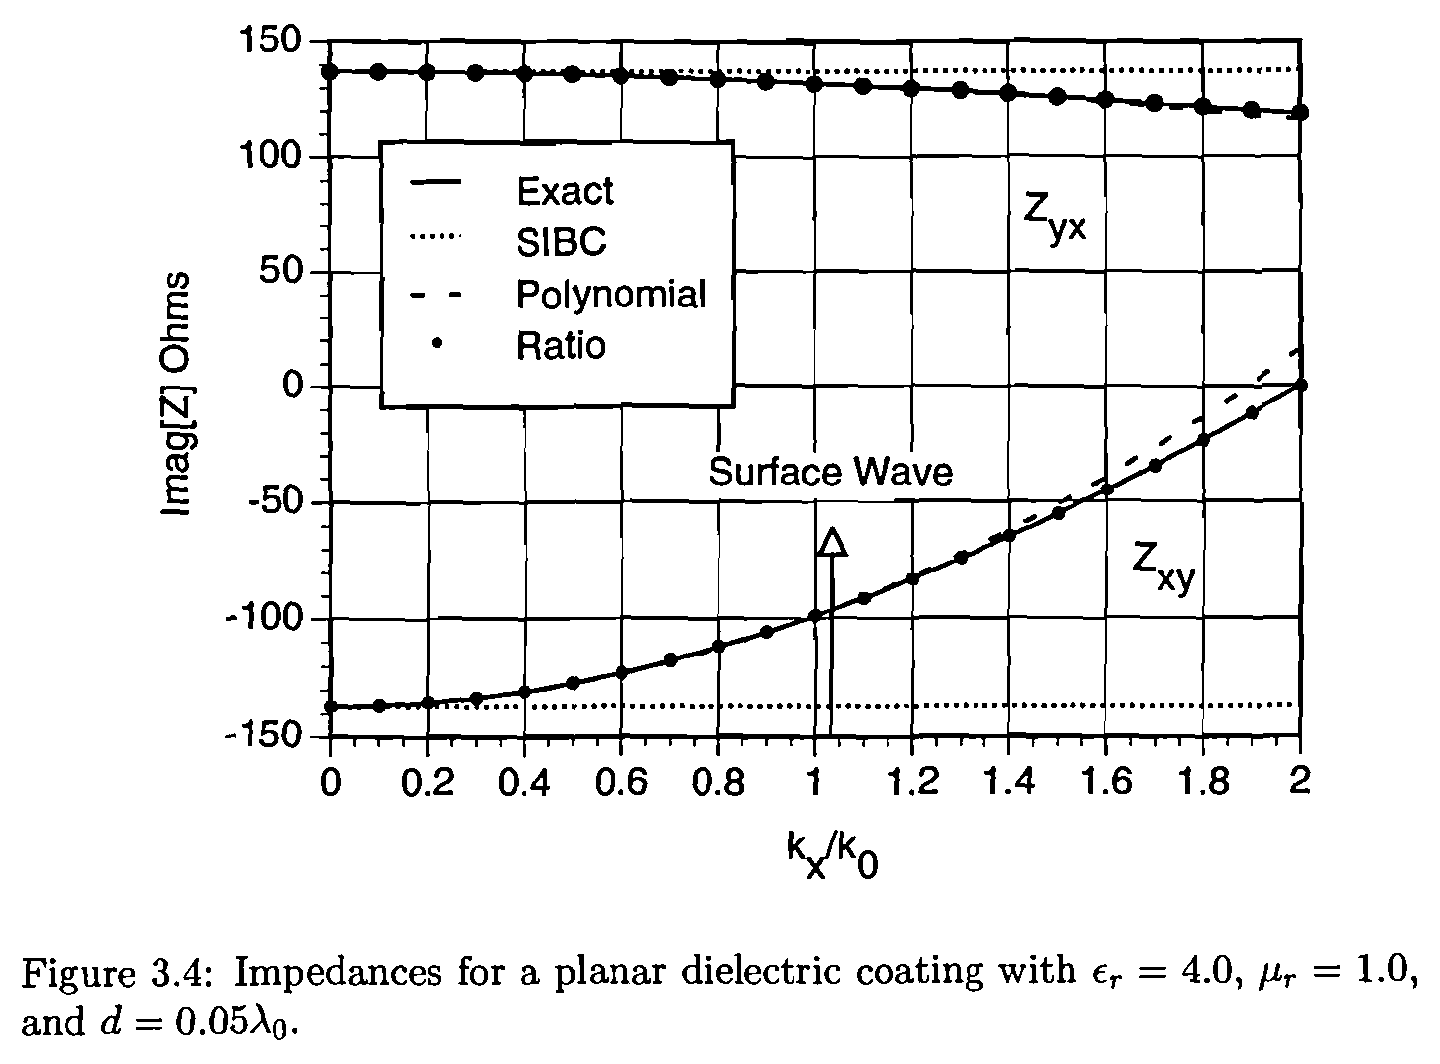
\includegraphics[width=0.99\textwidth]{images/hoppe/p33_imp_cylindre.png}
    \caption{Courbes de la page 33 de Hoppe Rahmat-Samii 1995}
    \label{fig:annex:hoppe:p33}
\end{figure}

La figure \ref{fig:annex:hoppe:p62} représente la partie imaginaire du symbole de l'opérateur d'impédance  pour un cylindre. La courbe \textit{Exact} correspond au symbole, \textit{HOIBC Planar} à la CIOE CI3 et \textit{HOIBC Curvature} à la CIOE CI6.

\begin{figure}[h!tb]
    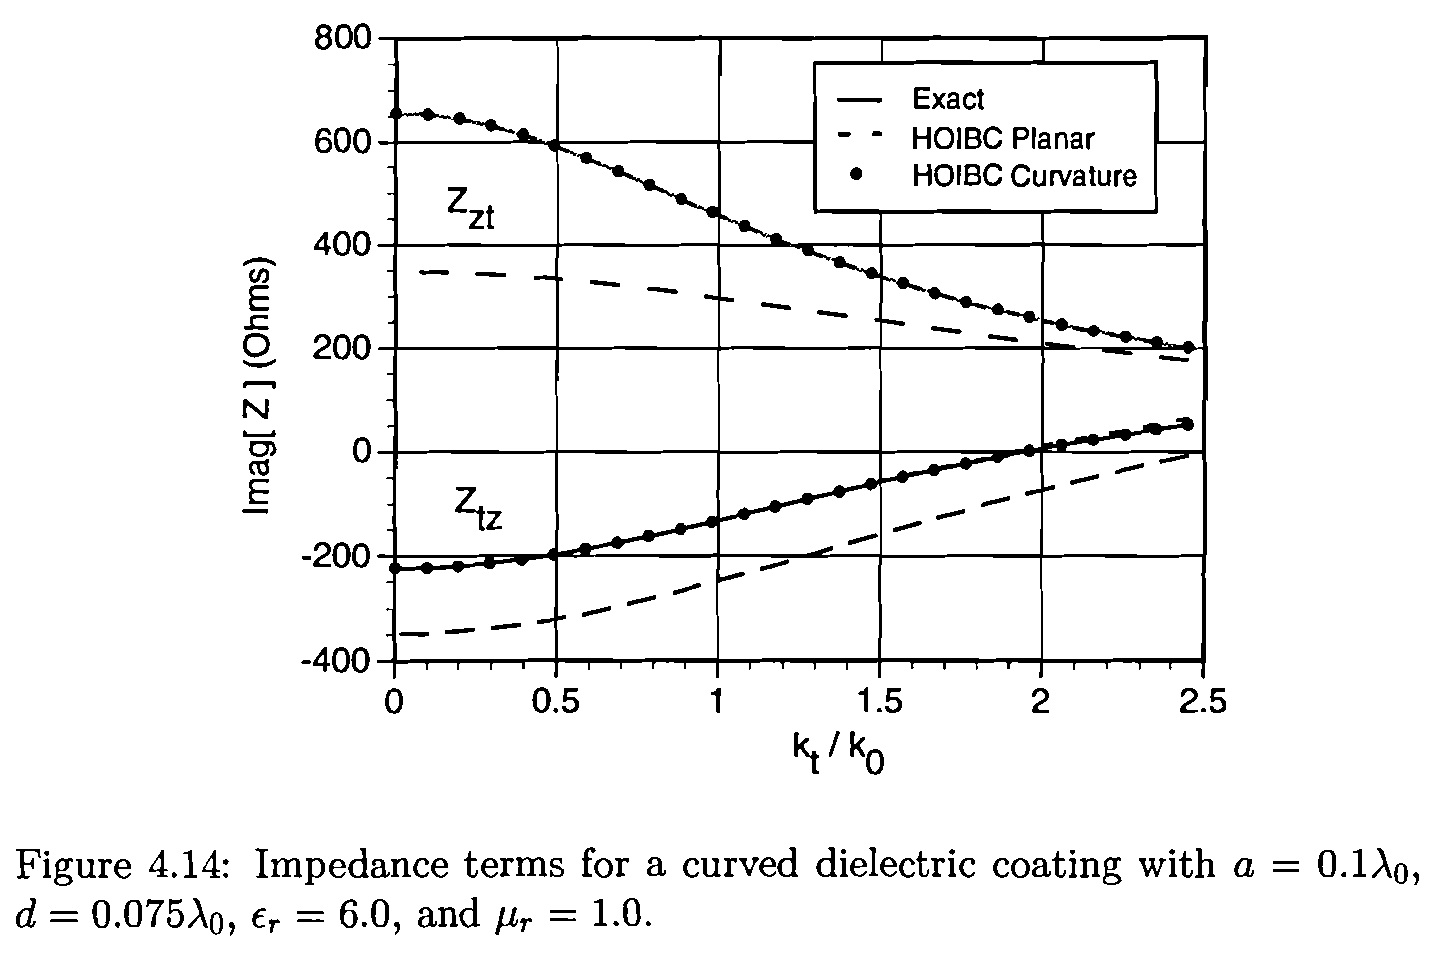
\includegraphics[width=0.99\textwidth]{images/hoppe/p62_imp_cylindre.png}
    \caption{Courbes de la page 62 de Hoppe Rahmat-Samii 1995}
    \label{fig:annex:hoppe:p62}
\end{figure}

\newpage
\section[Espaces Hdiv et Hrot]{Espaces \(\Hdiv\) et \(\Hrot\)}

Ces espaces ont été étudiés par \cite{nedelec_mixed_1980}. Nous rappelons dans cette annexe, les résultats principaux et les relations de compatibilité pour des fonctions de bases associées à ces espaces.

Soit \(\Gamma\) une surface fermée bornée régulière de \(\RR^3\).
Soit \(\Gamma_h\) une approximation de \(\Gamma\) par un maillage triangulaire, on désigne notamment un triangle de \(\Gamma_h\) par \(T\).

\begin{defn}
    Pour tout \(T \in \Gamma_h\), soit \(\phi_{|T}\) une fonction intégrable sur \(T\) alors
    on définit la notion de fonction intégrale sur \(\Gamma_h\), la fonction \(\phi_h\) telle que
    \begin{equation*}
        \int_{\Gamma_h} \phi_h \dd{\Gamma_h} = \sum_{T\in\Gamma_h} \int_T \phi_{|T} \dd{T}
    \end{equation*}
\end{defn}

\begin{defn}
    On dit que \(\phi_h \in L^2(\Gamma_h)\) si et seulement si \(\phi_{|T} \in L^2(T)\) pour tout \(T \in \Gamma_h\)
\end{defn}

\subsection[Hdiv]{\(\Hdiv\)}

\begin{defn}
    On dit que \(\vect{\Psi_h} \in \Hdiv(\Gamma_h)\) si et seulement si \(\vect{\Psi}_{|T} \in \Hdiv(T)\) pour tout \(T \in \Gamma_h\)
    Alors on définit sous forme faible \(\vdivs \vect{\Psi_h} \).
    Soit \(\phi \in C^1(\Gamma)\)
    \begin{equation*}
        \left< \vdivs \vect{\Psi_h}, \phi \right> %\int_{\Gamma_h} \vdivs \vect{\Psi_h} \phi \dd{\Gamma_h}
        = - \sum_{T\in\Gamma_h} \int_T \vect{\Psi}_{|T} \cdot \vgrads \phi\dd{T}
    \end{equation*}
\end{defn}

Autrement dit, \cite[eq.~5.3]{bendali_equations_2014}
\begin{defn}
    On dit que \(\vect{\Psi_h} \in \Hdiv(\Gamma_h)\) si et seulement s’ il existe \(\psi\in L^2(\Gamma)\) telle que pour toute \(\phi \in C^1(\Gamma)\)
    \begin{equation*}
        \left< \vdivs \vect{\Psi_h}, \phi \right> = \int_\Gamma \psi \phi \dd{\Gamma}
    \end{equation*}
\end{defn}

On déduit la relation de compatibilité \(\Hdiv\) suivante (\cite[Lemme.~8]{nedelec_mixed_1980})
\begin{prop}
    \label{prop:annex:hdiv_hrot:hdiv}
    Soit \(\vect{\Psi}\) tel que \(\vect{\Psi}_{|T}\) soit régulier pour tout \(T\in\Gamma_h\).\\
    Alors \(\vect{\Psi} \in \Hdiv(\Gamma_h)\) si et seulement si pour toute arête \(v_j\) séparant les triangles \(T_j^g\) et \(T_j^d\) où \(\vect{\nu}_j\) est le vecteur unitaire sortant du triangle \(T_j^g\) vers \(T_j^d\), on a
    \begin{equation*}
        \left( \vect{\Psi}_{|T_j^g} - \vect{\Psi}_{|T_j^d} \right ) \cdot \vect{\nu}_j = 0
    \end{equation*}
\end{prop}

\begin{proof}
    Cela se démontre grâce aux formules de Green pour la divergence surfacique (voir \cite[eq.~(A3.47)]{bladel_electromagnetic_2007}) en remarquant que la surface \(\Gamma_h\) est fermée et qu'un triangle possède toujours une arête en commun avec un autre.

    \begin{align*}
    \left< \vdivs \vect{\Psi_h}, \phi \right>
    & = - \sum_{T\in\Gamma_h} \int_T \vect{\Psi}_{|T} \cdot \vgrads \phi\dd{T} \\
    & = \sum_{T\in\Gamma_h} \int_T \vdivs \vect{\Psi}_{|T} \phi \dd{T} - \sum_{T\in\Gamma_h} \int_{\partial T} \vect{\Psi}_{|T} \cdot \nu_T \phi \dd{\gamma} \\
    & = \int_\Gamma \psi \phi \dd{\Gamma} - \sum_{T\in\Gamma_h} \int_{\partial T} \vect{\Psi}_{|T} \cdot \nu_T \phi \dd{\gamma} \\
    & = \int_\Gamma \psi \phi \dd{\Gamma} - \sum_{j=1}^{N_{vj}} \int_{v_j} \left( \vect{\Psi}_{|T_j^g} - \vect{\Psi}_{|T_j^d} \right) \cdot \nu_j \phi \dd{\gamma}
    \end{align*}
\end{proof}

\subsection[Hrot]{\(\Hrot\)}

L'espace \(\Hrot\) a déjà été étudié par \cite[Lemme.~ 6]{nedelec_mixed_1980}. Nous rappelons les résultats de compatibilité et leurs démonstrations.

\begin{defn}
    On dit que \(\vect{\Psi_h} \in \Hrot(\Gamma_h)\) si et seulement si \(\vect{\Psi}_{|T} \in \Hrot(T)\) pour tout \(T \in \Gamma_h\).\\
    Alors on définit sous forme faible \(\vrots \vect{\Psi_h} \).
    Soit \(\phi \in C^1(\Gamma)\)
    \begin{equation*}
        \left< \vn_\Gamma \cdot \vrots \vect{\Psi_h}, \phi \right> %\int_{\Gamma_h} \vdivs \vect{\Psi_h} \phi \dd{\Gamma_h}
        = - \sum_{T\in\Gamma_h} \int_T \vect{\Psi}_{|T}  \cdot \left( \vn_T \pvect \vgrads \phi \right) \dd{T}
    \end{equation*}
\end{defn}

On déduit la relation de compatibilité \(\Hrot\) suivante
\begin{prop}
    \label{prop:annex:hdiv_hrot:hrot}
    Soit \(\vect{\Psi}\) tel que \(\vect{\Psi}_{|T}\) soit régulier pour tout \(T\in\Gamma_h\).\\
    Alors \(\vect{\Psi} \in \Hrot(\Gamma_h)\) si et seulement si pour toute arête \(v_j\) séparant les triangles \(T_j^g\) et \(T_j^d\) où \(\vect{\nu}_j\) est le vecteur unitaire sortant du triangle \(T_j^g\) vers \(T_j^d\), et \(\tau_j = \vn_T \pvect \nu_j\) on a
    \begin{equation*}
        \left(\vect{\Psi}_{|T_j^g} - \vect{\Psi}_{|T_j^d} \right) \cdot \tau_j = 0
    \end{equation*}
\end{prop}

De même que pour \(\Hdiv\), cela ce démontre grâce aux formules de Green pour le rotationnel surfacique (voir \cite[eq.~(A3.57)]{bladel_electromagnetic_2007}) en remarquant que la surface \(\Gamma_h\) est fermée et qu'un triangle possède toujours une arête en commun avec un autre.

\begin{proof}
    \begin{align*}
    \left< \vn_\Gamma \cdot \vrots \vect{\Psi_h}, \phi \right>
    & = - \sum_{T\in\Gamma_h} \int_T \vect{\Psi}_{|T}  \cdot \left( \vn_T \pvect \vgrads \phi \right) \dd{T} \\
    & = \sum_{T\in\Gamma_h} \int_T \vn_T \cdot \vrots \vect{\Psi}_{|T} \phi \dd{T} - \sum_{T\in\Gamma_h} \int_{\partial T}  \vect{\Psi}_{|T} \cdot \left(\vn_T \pvect \nu_T \right)\phi\dd{\gamma}\\
    & = \int_\Gamma \psi \phi \dd{\Gamma} - \sum_{T\in\Gamma_h} \int_{\partial T}  \vect{\Psi}_{|T} \cdot \tau_j \phi\dd{\gamma}\\
    &= \int_\Gamma \psi \phi \dd{\Gamma} - \sum_{j=1}^{N_{vj}} \int_{v_j}  \left(\vect{\Psi}_{|T_j^g} - \vect{\Psi}_{|T_j^d} \right) \cdot \tau_j \phi\dd{\gamma}
    \end{align*}
\end{proof}

